\documentclass[10pt,twocolumn,letterpaper]{article}

\usepackage{cvpr}
\usepackage{times}
\usepackage{epsfig}
\usepackage{graphicx, color, xcolor}
\usepackage{amsmath}
\usepackage{amssymb}
\usepackage{bm}
\usepackage[utf8]{inputenc}
\usepackage{fancyhdr}
\usepackage[brazil, english]{babel}
\setlength{\headheight}{1.5cm}
\usepackage{float}
\usepackage{listings}
\usepackage{booktabs}
\usepackage{array}
\raggedbottom

\fancypagestyle{plain}{%\fancyhf{}%}
\lhead{
\includegraphics[width=5cm,height=2cm]{logoFT.png}}
\rhead{
\includegraphics[width=5cm,height=2cm]{logoUnB.png}}

\renewcommand{\headrulewidth}{1pt}%
}

% Changing the caption and 'References' names to Portuguese.
\addto\captionsenglish{
  \renewcommand{\figurename}{Figura}
  \renewcommand{\tablename}{Tabela}
  \renewcommand{\refname}{Referências bibliográficas}
}
\renewcommand{\lstlistingname}{Código}

\hyphenation{co-e-ren-te u-sa-do de-li-mi-ta-do-res a-cer-ca va-lo-res cor-res-pon-den-te re-fe-ren-ci-a-das co-lu-na co-lu-nas em-bo-ra u-ti-li-da-de pro-ce-di-men-to ex-pe-ri-men-to fi-gu-ras}

\usepackage[breaklinks=true,bookmarks=true]{hyperref}

\definecolor{codebg}{RGB}{245,245,245}
\lstset{
  backgroundcolor=\color{codebg},
  basicstyle=\ttfamily\scriptsize,
  breaklines=true,
  frame=single,
  numbers=left,
  numberstyle=\tiny,
  keywordstyle=\color{blue!70!black}\bfseries,
  commentstyle=\color{green!40!black},
  stringstyle=\color{red!60!black},
  showstringspaces=false,
  language=Python
}

\cvprfinalcopy % *** Uncomment this line for the final submission

\begin{document}
%%%%%%%%% TITLE
\title{Trabalho 1, Introdução ao Processamento de Imagens}

\author{Marcos Paulo de Oliveira\\
{\tt\small 221020889@aluno.unb.br}\\
{\tt\small 22/1020889}
}

\maketitle

%%%%%%%%% OBJETIVO
\begin{objetivo}
O objetivo deste trabalho é implementar e avaliar técnicas de processamento
digital de imagens em duas frentes: (1) aumento do tamanho de imagens por
repetição de pixels, por interpolação com média e por combinação
(entrelaçamento) de duas imagens em uma de maior resolução; e (2) realce de
contraste por transformação \emph{power-law} (correção gamma) e por
equalização de histograma. Todo o código foi desenvolvido em Python,
utilizando as bibliotecas NumPy e OpenCV.
\end{objetivo}

%%%%%%%%% BODY TEXT
\section{Introdução}

Este relatório documenta a implementação do Trabalho 1 da disciplina de
Introdução ao Processamento de Imagens. A Questão 1 trata de três funções de
manipulação geométrica de imagens: \texttt{TAM2} (aumento por repetição de
pixels), \texttt{TAMM} (aumento por interpolação com média) e
\texttt{SUPERRES} (combinação de duas imagens em uma de maior resolução). A
Questão 2 trata de realce de contraste através de duas técnicas clássicas:
\emph{power-law} (correção gamma) e equalização de histograma.

Em substituição às imagens padrão \texttt{FRUIT1.jpg} e \texttt{FRUIT2.jpg}
sugeridas no enunciado para a Questão 1, utilizamos duas fotografias
próprias, recortadas ao centro em formato quadrado e redimensionadas para
$300\times300$ pixels. Para a Questão 2, utilizamos as imagens fornecidas
\texttt{car.png} ($600\times338$), \texttt{crowd.png} ($800\times600$) e
\texttt{university.png} ($399\times300$).

%-------------------------------------------------------------------------
\section{Questão 1, Aumento e combinação de imagens}

\begin{figure}[H]
  \centering
  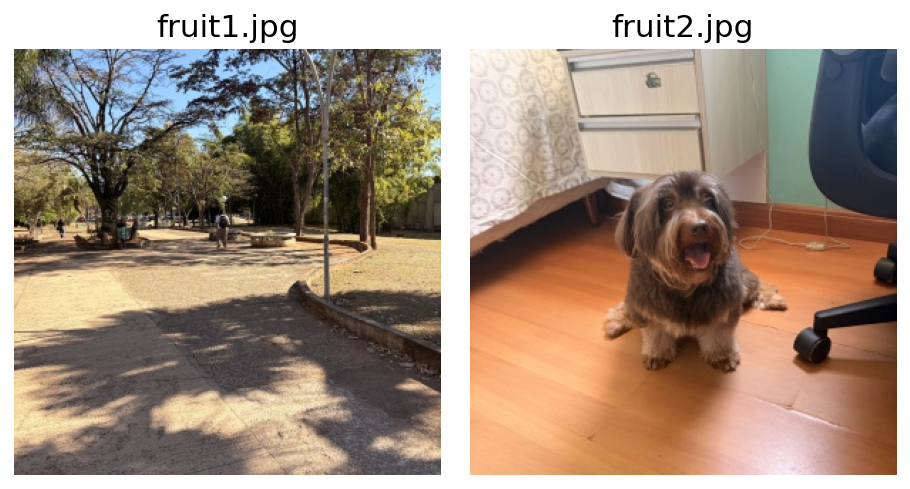
\includegraphics[width=\linewidth]{figs/painel_originais.png}
  \caption{Imagens originais utilizadas na Questão 1 (substitutas de
  FRUIT1.jpg e FRUIT2.jpg).}
  \label{fig:originais}
\end{figure}

\subsection{Função TAM2}

A função \texttt{TAM2(img, n)} aumenta uma imagem RGB em $n$ vezes (linhas e
colunas), repetindo cada linha e cada coluna originais, conforme o exemplo do
enunciado. Seguindo a dica do enunciado, implementamos uma função auxiliar
\texttt{aumenta2} que dobra o tamanho da imagem, e a chamamos repetidamente
dentro de \texttt{TAM2} até atingir o fator desejado (ex.: para $n=8$,
\texttt{aumenta2} é chamada 3 vezes, pois $2^3=8$).

\begin{lstlisting}[caption={Função TAM2 (arquivo \texttt{src/tam2.py}).}]
def aumenta2(img):
    """Duplica cada linha e cada coluna da imagem (fator de aumento = 2)."""
    dobrado_linhas = np.repeat(img, 2, axis=0)
    dobrado = np.repeat(dobrado_linhas, 2, axis=1)
    return dobrado

def TAM2(img, n):
    if n < 2 or n % 2 != 0:
        raise ValueError("n deve ser par e >= 2.")
    resultado = img.copy()
    fator_restante = n
    while fator_restante % 2 == 0:
        resultado = aumenta2(resultado)
        fator_restante //= 2
    if fator_restante > 1:
        resultado = repete_fator(resultado, fator_restante)
    return resultado
\end{lstlisting}

Validamos a função contra o exemplo numérico do enunciado ($2\times2 \to
4\times4$, fator 2) e o resultado foi idêntico pixel a pixel ao esperado.

\begin{figure}[H]
  \centering
  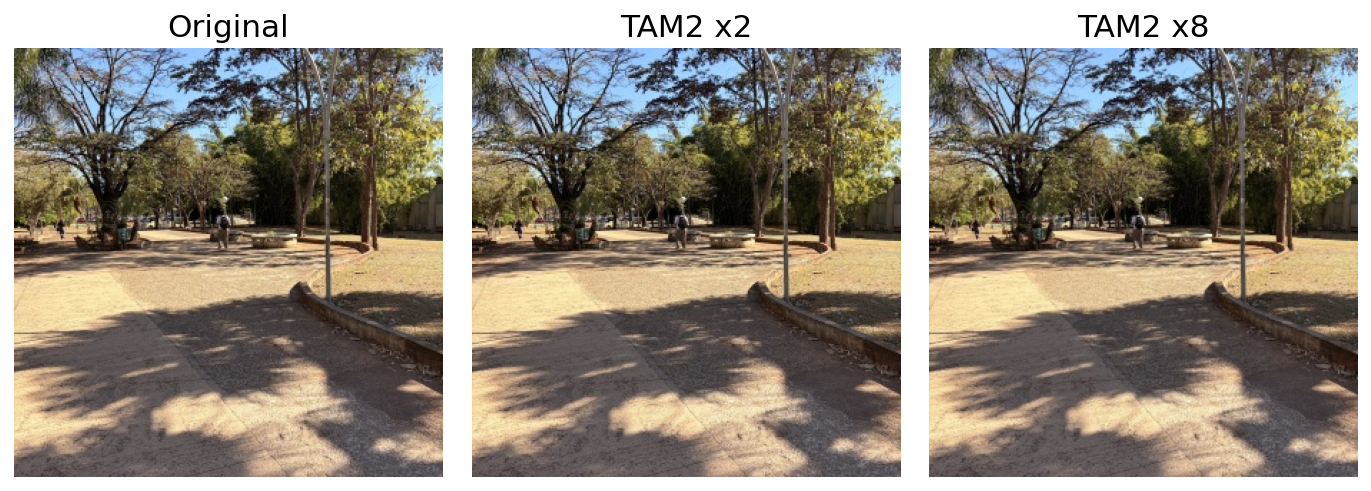
\includegraphics[width=\linewidth]{figs/painel_tam2.png}
  \caption{Resultado de TAM2 aplicado a fruit1.jpg, com fatores 2 e 8.}
  \label{fig:tam2}
\end{figure}

\textbf{Comentários (fruit1.jpg):} em ambos os fatores (2 e 8, Figura
\ref{fig:tam2}) a imagem aumentada preserva perfeitamente as cores e o
conteúdo da imagem original, pois nenhuma informação é perdida, apenas
repetida. No entanto, como o método usado é a repetição do vizinho mais
próximo (\emph{nearest neighbor}), o resultado apresenta um nítido efeito de
``blocos'' (pixelização), que fica muito mais evidente quanto maior o fator
de aumento. Com fator 2 o efeito é discreto e quase imperceptível a
distância normal de visualização; já com fator 8 as bordas da imagem
(galhos, folhas) ficam visivelmente serrilhadas. Isso ocorre porque TAM2 não
introduz nenhuma informação nova entre os pixels originais, ele apenas os
replica (comparamos essa pixelização diretamente com o resultado de TAMM,
de forma ampliada, na próxima seção).

\subsection{Função TAMM}

A função \texttt{TAMM(img)} também aumenta a imagem em 2 vezes, mas em vez de
repetir os pixels, utiliza a \textbf{média} entre pixels vizinhos (quando
possível). O preenchimento ocorre em duas passadas, conforme o enunciado:
(1) os pixels ``vermelhos'' preenchem as colunas intermediárias das linhas
que já contêm pixels originais, usando a média horizontal entre o pixel à
esquerda e o pixel à direita (quando não há vizinho à direita, na última
coluna, repete-se o valor anterior); (2) os pixels ``azuis'' preenchem as
linhas totalmente vazias, usando a média vertical entre a linha de cima e a
linha de baixo, já preenchidas no passo anterior (quando não há linha
abaixo, na última linha, repete-se a linha de cima).

\begin{lstlisting}[caption={Núcleo da função TAMM (arquivo \texttt{src/tamm.py}).}]
out[0::2, 0::2, :] = img  # pixels originais

# Passo 1: colunas impares das linhas pares -> media horizontal
for j in range(1, 2*w, 2):
    if j + 1 < 2*w:
        out[0::2, j, :] = round_half_up((out[0::2, j-1, :] + out[0::2, j+1, :]) / 2)
    else:
        out[0::2, j, :] = out[0::2, j-1, :]

# Passo 2: linhas impares (vazias) -> media vertical
for i in range(1, 2*h, 2):
    if i + 1 < 2*h:
        out[i, :, :] = round_half_up((out[i-1, :, :] + out[i+1, :, :]) / 2)
    else:
        out[i, :, :] = out[i-1, :, :]
\end{lstlisting}

Um detalhe importante encontrado durante a validação: a função
\texttt{numpy.round} utiliza arredondamento ``bancário'' (0,5 arredonda para
o par mais próximo), o que faria $8{,}5 \to 8$, divergindo do exemplo do
enunciado (que espera $8{,}5 \to 9$). Por isso implementamos um
arredondamento ``0,5 sempre para cima'' (\texttt{floor(x + 0,5)}), que
reproduziu exatamente a matriz de exemplo do enunciado:

\[
\begin{pmatrix}10 & 12\\ 5 & 7\end{pmatrix}
\xrightarrow{\text{TAMM}}
\begin{pmatrix}10 & 11 & 12 & 12\\ 8 & 9 & 10 & 10\\ 5 & 6 & 7 & 7\\ 5 & 6 & 7 & 7\end{pmatrix}
\]

\begin{figure}[H]
  \centering
  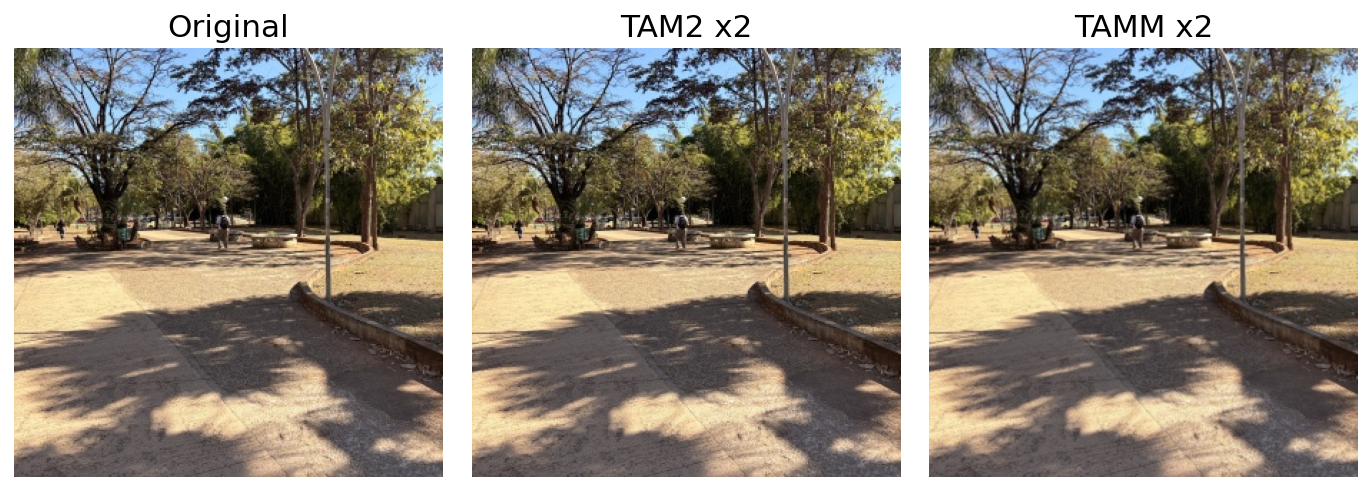
\includegraphics[width=\linewidth]{figs/painel_tam2_vs_tamm.png}
  \caption{Comparação entre TAM2 e TAMM, fator 2, em fruit1.jpg.}
  \label{fig:tamm}
\end{figure}

\begin{figure}[H]
  \centering
  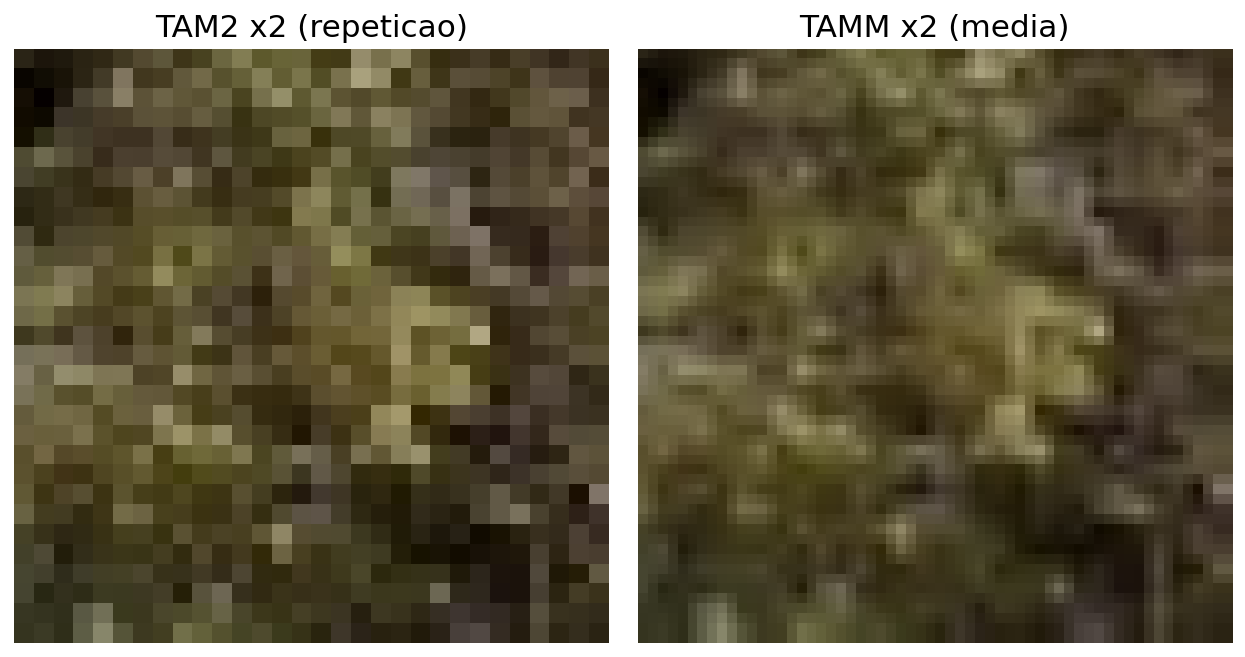
\includegraphics[width=\linewidth]{figs/painel_tam2_vs_tamm_zoom.png}
  \caption{Zoom (mesmo recorte de 30$\times$30) comparando o efeito de
  blocos do TAM2 com o suavizado do TAMM, fator 2.}
  \label{fig:tamm_zoom}
\end{figure}

\begin{figure}[H]
  \centering
  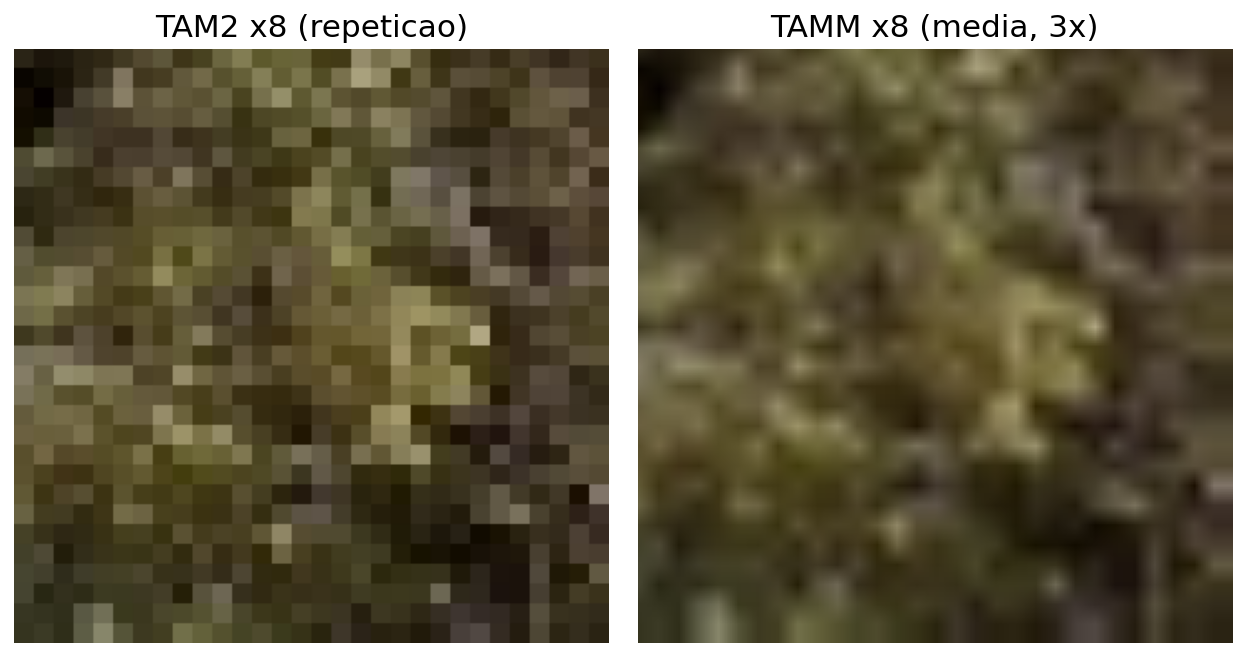
\includegraphics[width=\linewidth]{figs/painel_tam2_zoom.png}
  \caption{Mesmo recorte, agora no fator 8 (TAMM aplicada 3 vezes, já que a
  função só aumenta em 2 por chamada): a diferença entre repetição e média
  fica muito mais evidente nesse fator mais extremo.}
  \label{fig:tamm_zoom_x8}
\end{figure}

\textbf{Comparação TAM2 $\times$ TAMM:} como esperado, a imagem gerada por
TAMM é visivelmente mais suave do que a gerada por TAM2 (Figuras
\ref{fig:tamm}, \ref{fig:tamm_zoom} e \ref{fig:tamm_zoom_x8}). Como TAMM
interpola valores intermediários (em vez de apenas repetir), as transições
de cor/intensidade entre pixels vizinhos ficam mais graduais, reduzindo o
efeito de blocos observado no TAM2. No fator 2 (Figura~\ref{fig:tamm_zoom})
essa suavização já é perceptível, mas sutil; aplicando TAMM repetidamente
até o fator 8 (Figura~\ref{fig:tamm_zoom_x8}) o borramento se acumula a cada
passo e a diferença em relação aos blocos nítidos do TAM2 fica bastante
evidente. O custo é esse mesmo efeito de borramento (\emph{blur}) nas
bordas mais nítidas da imagem, já que a média tende a atenuar transições
bruscas de intensidade. Em termos de qualidade visual percebida, o
resultado de TAMM é geralmente preferível ao de TAM2 para aumento de
imagens naturais, pois produz uma aparência mais próxima de uma imagem
capturada originalmente naquela resolução, enquanto TAM2 deixa evidente que
a imagem foi artificialmente ampliada.

\emph{Nota sobre as comparações acima:} não incluímos o recorte original
lado a lado, porque ao exibir uma imagem pequena (30$\times$30) numa área
maior, qualquer visualizador faz exatamente a mesma ampliação por vizinho
mais próximo que o TAM2 faz, ou seja, os dois ficariam visualmente
idênticos, não por erro, mas porque matematicamente são a mesma operação.
A comparação que de fato revela alguma diferença é TAM2 contra TAMM, já
que essas duas funções produzem valores de pixel realmente diferentes.

\subsection{Função SUPERRES}

A função \texttt{SUPERRES(img1, img2)} combina duas imagens de mesmo tamanho
$H\times W$ em uma única imagem $2H\times2W$, posicionando os pixels de
\texttt{img1} nas posições de linha e coluna \emph{ímpares} (indexação
MATLAB, 1-based) e os pixels de \texttt{img2} nas posições \emph{pares}.
Validamos o posicionamento contra os seis exemplos de coordenadas dados no
enunciado e todos bateram exatamente.

O enunciado não especifica o que fazer com as posições restantes do
``tabuleiro de xadrez'' resultante (linha par/coluna ímpar e linha
ímpar/coluna par). Adotamos a solução de preencher essas posições pela
\textbf{média dos vizinhos diretos já conhecidos} (cima, baixo, esquerda e
direita, ou os que existirem nas bordas), no mesmo espírito de
preenchimento por média usado na função TAMM.

\begin{lstlisting}[caption={Núcleo da função SUPERRES (arquivo \texttt{src/superres.py}).}]
out[0::2, 0::2, :] = img1   # posicoes (linha,col) impares - 1-based (MATLAB)
out[1::2, 1::2, :] = img2   # posicoes (linha,col) pares   - 1-based (MATLAB)

# posicoes restantes: media dos vizinhos diretos (cima/baixo/esq/dir)
for r, c in posicoes_vazias:
    vizinhos = [out[r-1,c], out[r+1,c], out[r,c-1], out[r,c+1]]  # os que existirem (bordas)
    out[r, c, :] = round_half_up(mean(vizinhos))
\end{lstlisting}

\begin{figure}[H]
  \centering
  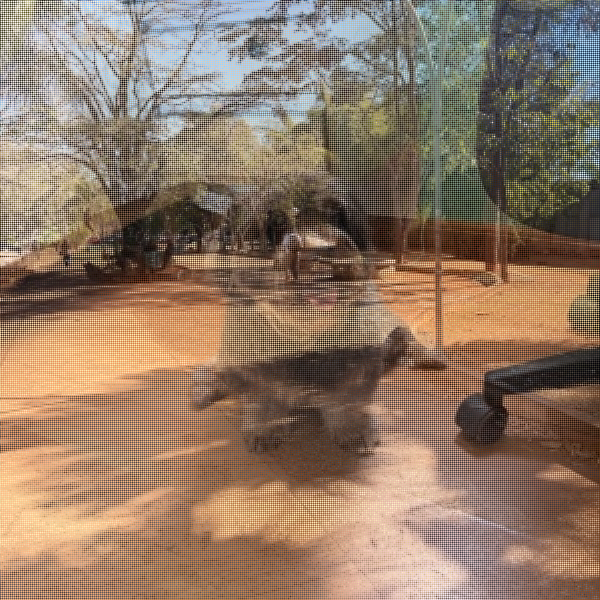
\includegraphics[width=\linewidth]{figs/fruit_superres.png}
  \caption{Resultado de SUPERRES(fruit1, fruit2), imagem $600\times600$
  combinando as duas fotos $300\times300$.}
  \label{fig:superres}
\end{figure}

\textbf{Comentários:} diferentemente de TAM2 e TAMM, que aumentam uma única
imagem, SUPERRES \emph{entrelaça duas imagens distintas}. O resultado
(Figura~\ref{fig:superres}) deixa isso evidente: como fruit1.jpg e
fruit2.jpg são fotos completamente diferentes (não duas capturas
sub-pixel deslocadas da mesma cena, como seria necessário em um cenário real
de super-resolução), a imagem final apresenta um padrão visível de
``tabuleiro''/\emph{moiré}, misturando o conteúdo das duas fotos em vez de
reconstruir uma imagem única de maior resolução e nitidez. Isso ilustra bem
o princípio por trás da super-resolução por múltiplos quadros: a técnica só
funciona quando as duas imagens de entrada são amostras levemente deslocadas
(sub-pixel) da \emph{mesma} cena, nesse caso, cada imagem preenche
``buracos'' de amostragem da outra, e o entrelaçamento reconstrói detalhes
que nenhuma das duas imagens individualmente possuía. Com duas cenas
diferentes, como usamos aqui, o entrelaçamento apenas sobrepõe informação
incompatível, resultando no efeito de interferência visível. Comparado a
TAM2 e TAMM (que, embora aumentem o tamanho, não acrescentam detalhe real),
SUPERRES mostra o maior potencial de ganho de qualidade, mas apenas quando
usado com o tipo de par de imagens adequado.

%-------------------------------------------------------------------------
\section{Questão 2, Realce de contraste: power-law e equalização}

Nesta questão aplicamos duas técnicas clássicas de realce de contraste sobre
as imagens em tons de cinza \texttt{car.png}, \texttt{crowd.png} e
\texttt{university.png}, usando as funções do OpenCV sugeridas no enunciado
(\texttt{cv2.pow}/\texttt{cv2.convertScaleAbs}, equivalentes a
\texttt{cvPow}/\texttt{cvConvertScaleAbs}, e \texttt{cv2.equalizeHist}).

\subsection{Realce power-law (correção gamma)}

A transformação power-law é dada por $s = c \cdot r^{\gamma}$, com $r$ (nível
de entrada) normalizado em $[0,1]$ e $c=255$. Testamos, para cada imagem,
pelo menos dois valores de $\gamma$ maiores que 1 e dois menores que 1,
escolhidos a partir da inspeção visual de cada imagem: \textbf{car.png}
(imagem muito clara/``estourada''): $\gamma=0{,}6$ (clareia ainda mais,
ruim), $\gamma=3{,}0$ e $\gamma=5{,}0$ (escurecem, aumentando o contraste);
\textbf{crowd.png} (imagem escura): $\gamma=0{,}3$, $\gamma=0{,}5$
(clareiam) e $\gamma=2{,}0$ (escurece ainda mais, ruim);
\textbf{university.png} (cena noturna, muito escura): $\gamma=0{,}2$,
$\gamma=0{,}4$ (clareiam) e $\gamma=2{,}0$ (escurece ainda mais, ruim).

\begin{lstlisting}[caption={Função de realce power-law (arquivo \texttt{src/q2\_main.py}).}]
def power_law(img_gray, gamma):
    normalizada = img_gray.astype(np.float64) / 255.0
    realcada = cv2.pow(normalizada, gamma)
    return cv2.convertScaleAbs(realcada, alpha=255.0)
\end{lstlisting}

\begin{figure}[H]
  \centering
  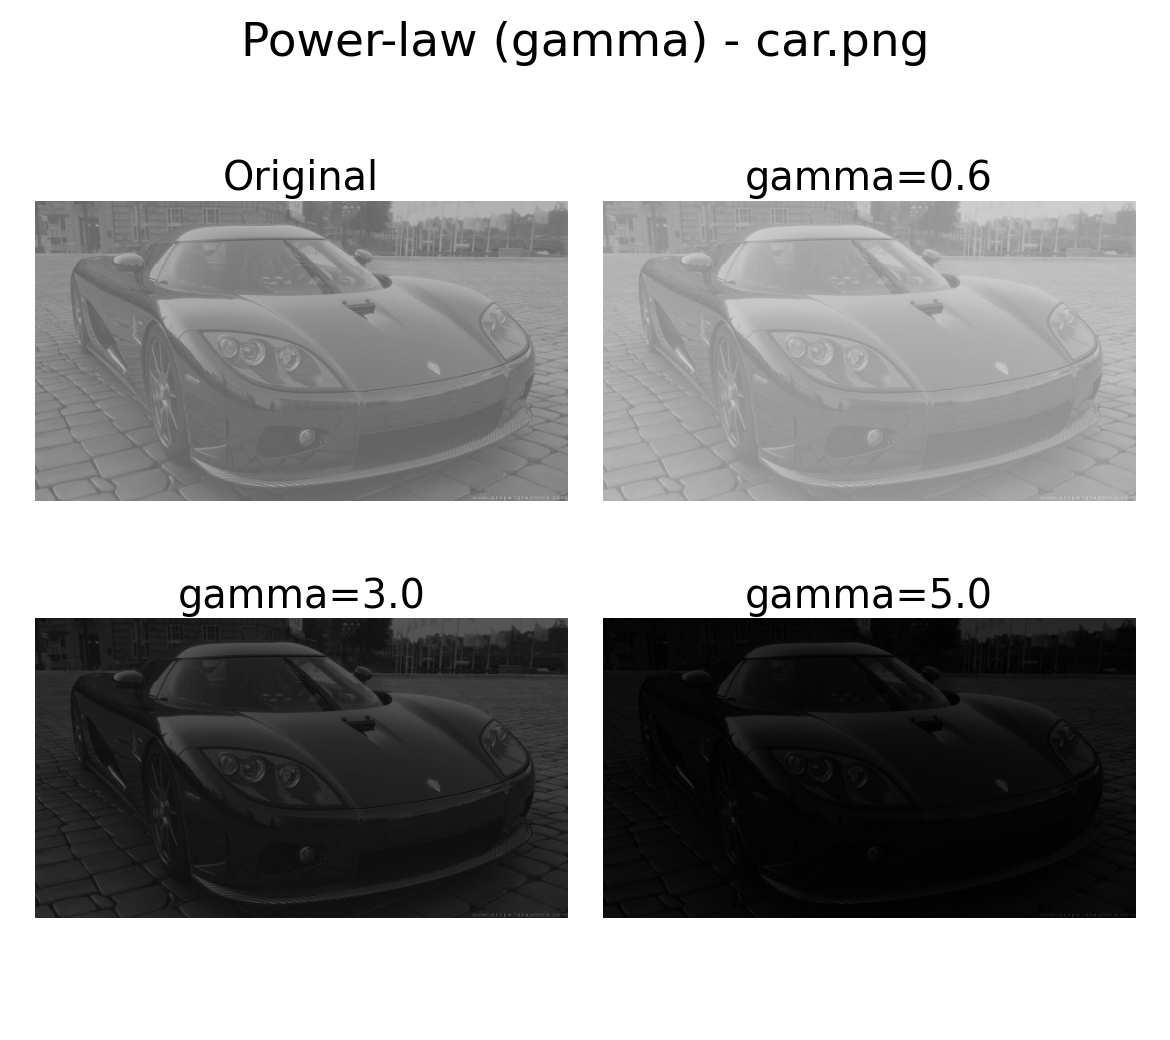
\includegraphics[width=\linewidth]{figs/car_gamma_comparativo.png}
  \caption{car.png, original e três valores de $\gamma$ testados.}
  \label{fig:car_gamma}
\end{figure}

\begin{figure}[H]
  \centering
  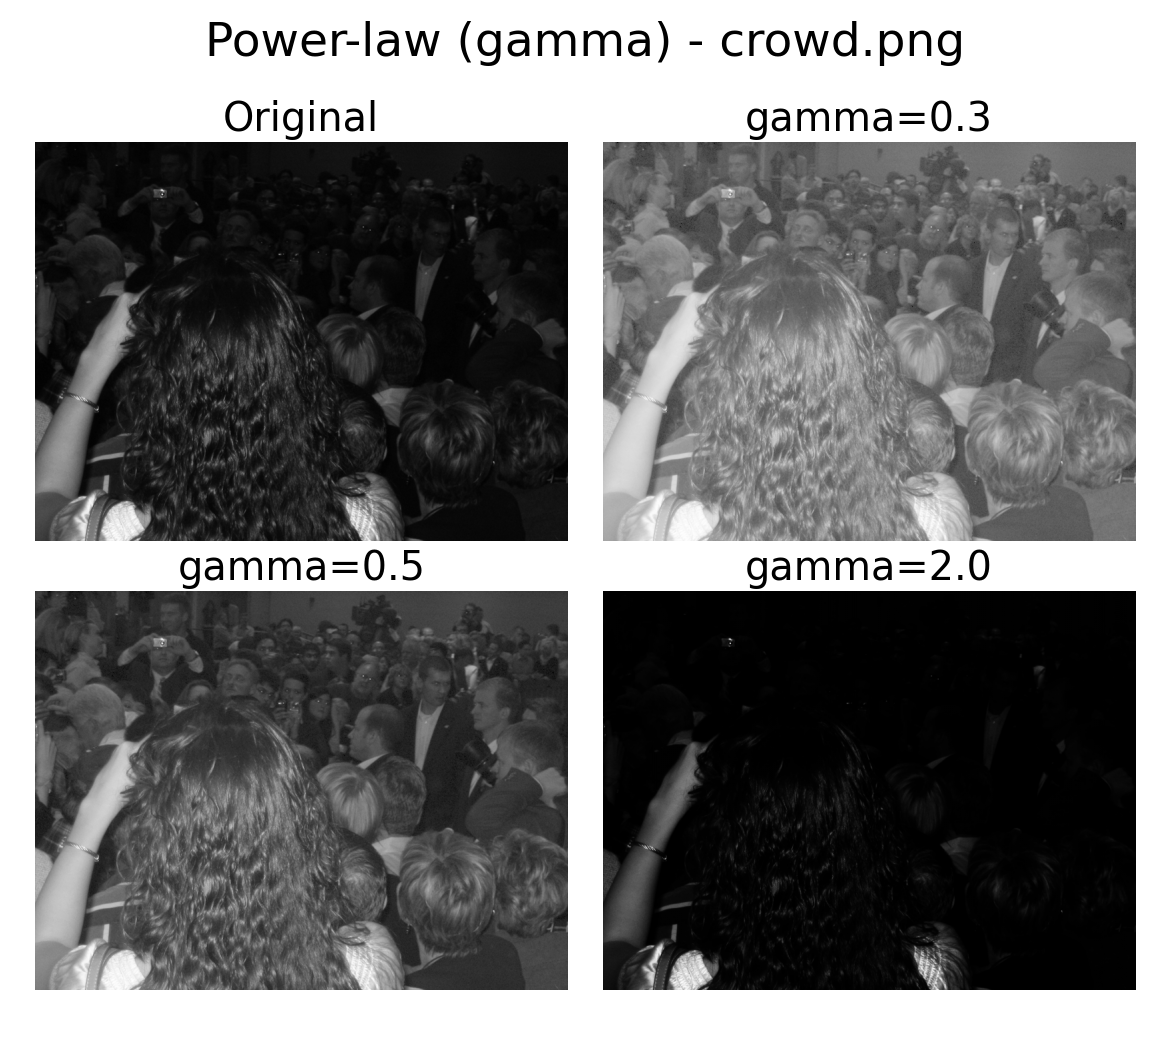
\includegraphics[width=\linewidth]{figs/crowd_gamma_comparativo.png}
  \caption{crowd.png, original e três valores de $\gamma$ testados.}
  \label{fig:crowd_gamma}
\end{figure}

\begin{figure}[H]
  \centering
  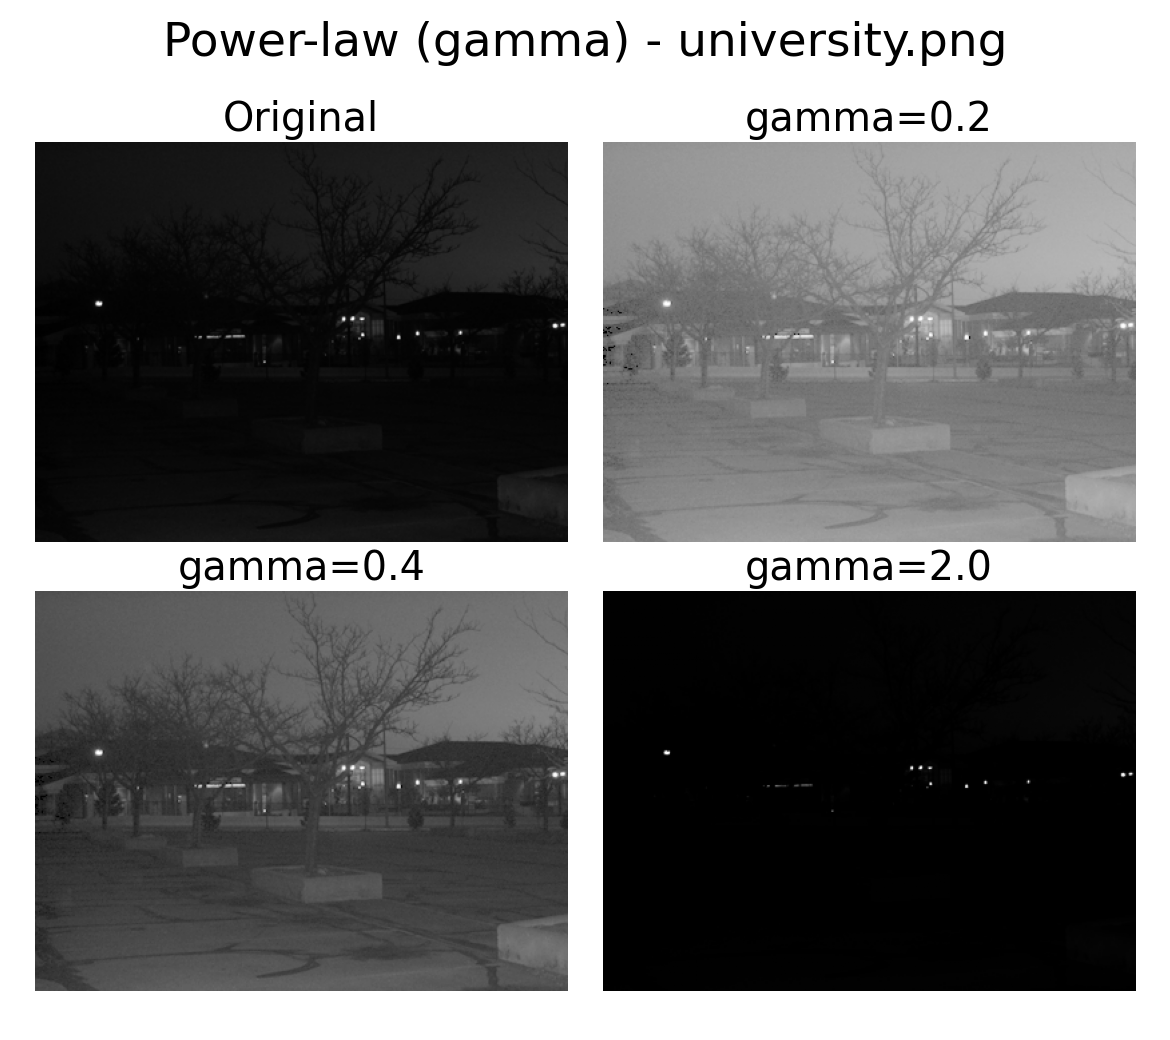
\includegraphics[width=\linewidth]{figs/university_gamma_comparativo.png}
  \caption{university.png, original e três valores de $\gamma$ testados.}
  \label{fig:university_gamma}
\end{figure}

\begin{table}[H]
  \centering
  \begin{tabular}{l c p{3cm}}
    \toprule
    Imagem & $\gamma$ & Justificativa \\
    \midrule
    car.png & $3{,}0$ & Recupera o contraste do carro sem perder detalhes do fundo \\
    crowd.png & $0{,}3$ & Revela rostos/roupas sem saturar as áreas já claras \\
    university.png & $0{,}4$ & Torna a cena noturna visível mantendo contraste \\
    \bottomrule
  \end{tabular}
  \caption{Melhor valor de $\gamma$ escolhido para cada imagem.}
  \label{tab:gamma}
\end{table}

\begin{figure}[H]
  \centering
  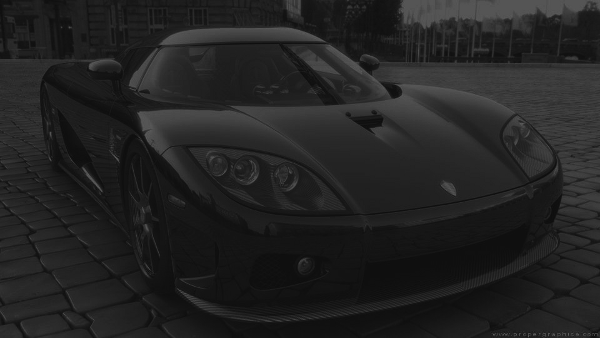
\includegraphics[width=\linewidth]{figs/car_melhor_gamma.png}
  \caption{car.png após power-law com o melhor $\gamma$ ($\gamma=3{,}0$).}
  \label{fig:car_melhor}
\end{figure}

\textbf{Comentários:} em todas as três imagens, valores de $\gamma < 1$
clareiam a imagem (expandem a faixa dos tons escuros, comprimem os tons
claros) e valores de $\gamma > 1$ a escurecem (efeito oposto). Como
\texttt{car.png} já é uma imagem muito clara (sobre-exposta), o melhor
resultado veio de $\gamma>1$; já \texttt{crowd.png} e
\texttt{university.png}, originalmente escuras, melhoraram com $\gamma<1$.
Em \texttt{university.png} notamos que $\gamma=0{,}2$ clareia bastante mas
``lava'' um pouco a imagem (reduz o contraste geral), enquanto
$\gamma=0{,}4$ oferece um equilíbrio melhor entre visibilidade e contraste,
por isso foi escolhido como melhor resultado (Tabela~\ref{tab:gamma}). Em
todos os casos, valores de $\gamma$ mal escolhidos (na direção errada da
imagem) pioram bastante a visualização, levando a imagens quase totalmente
pretas ou totalmente brancas, sem acrescentar informação visual.

\subsection{Equalização de histograma}

Equalizamos as três imagens com \texttt{cv2.equalizeHist}, que redistribui
os níveis de cinza de forma a aproximar o histograma resultante de uma
distribuição uniforme.

\begin{figure}[H]
  \centering
  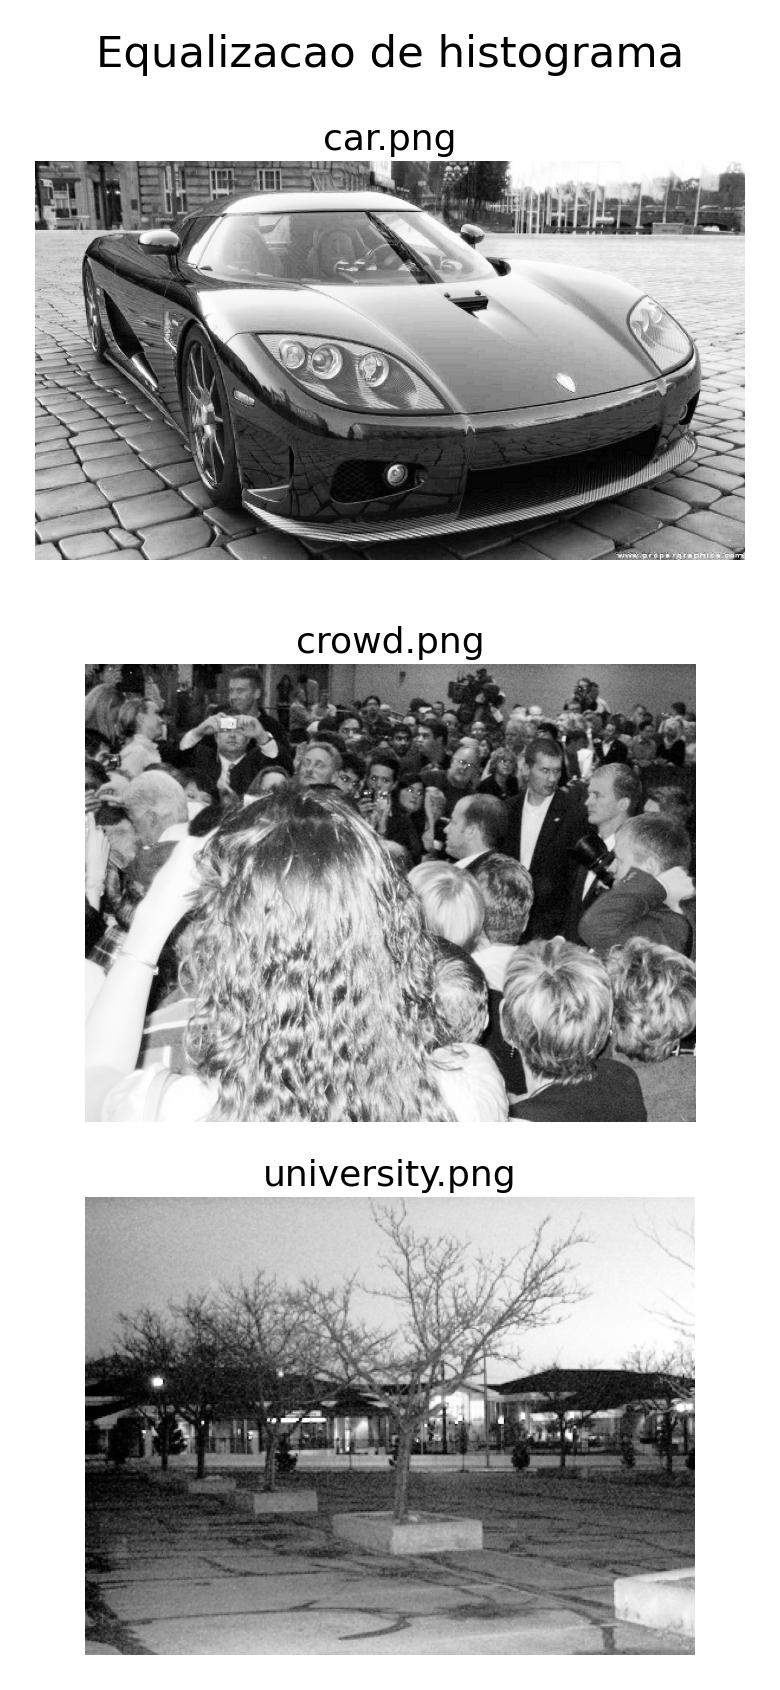
\includegraphics[width=\linewidth]{figs/todas_equalizadas.png}
  \caption{As três imagens após equalização de histograma.}
  \label{fig:todas_eq}
\end{figure}

Para \texttt{university.png} (a imagem mais escura, onde o efeito é mais
evidente), mostramos a comparação antes/depois e os respectivos histogramas
e funções de distribuição acumulada (CDF):

\begin{figure}[H]
  \centering
  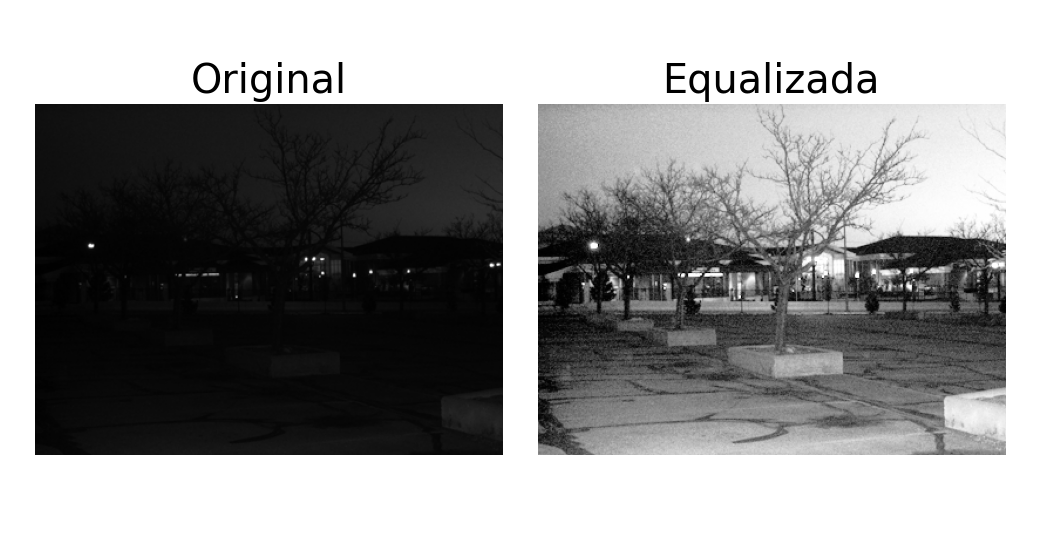
\includegraphics[width=\linewidth]{figs/university_antes_depois.png}
  \caption{university.png antes e depois da equalização de histograma.}
  \label{fig:univ_antes_depois}
\end{figure}

\begin{figure}[H]
  \centering
  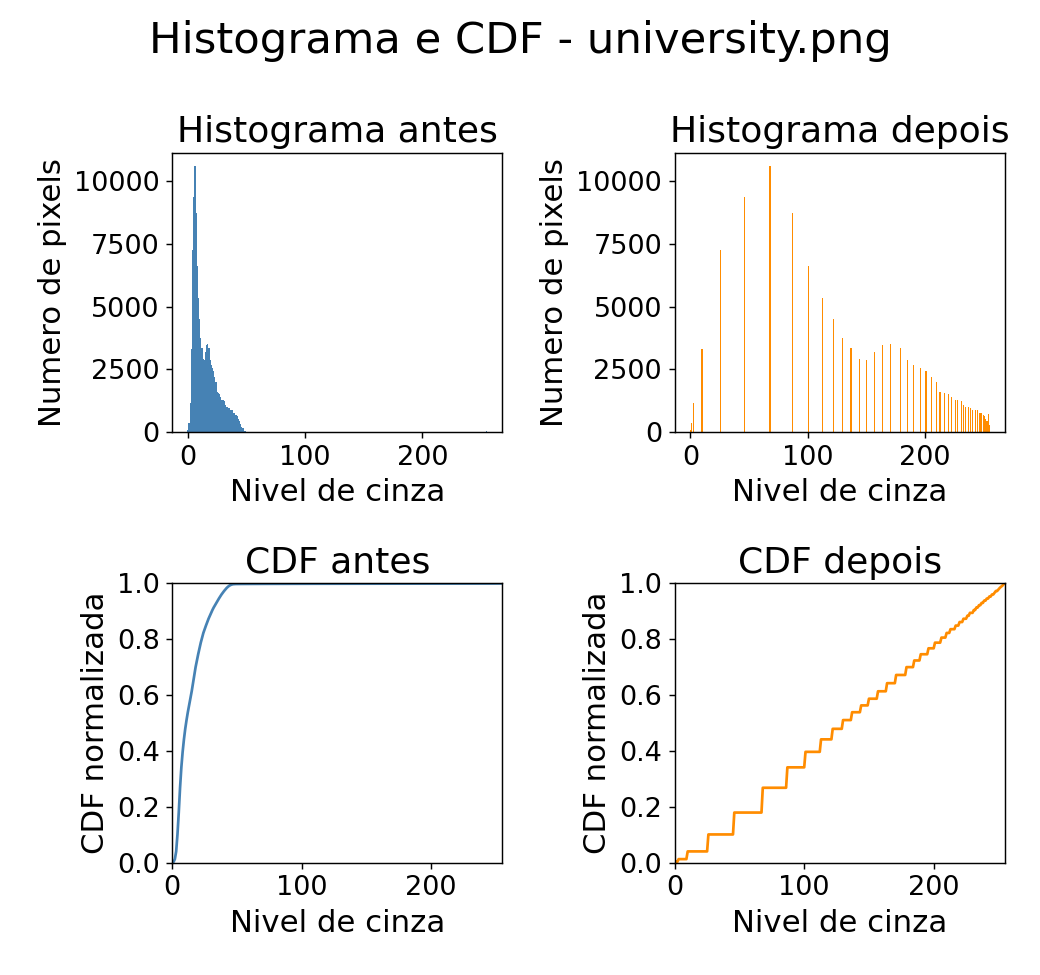
\includegraphics[width=\linewidth]{figs/university_hist_cdf.png}
  \caption{Histograma e CDF de university.png antes (esquerda) e depois
  (direita) da equalização.}
  \label{fig:hist_cdf}
\end{figure}

\textbf{Comentários:} o histograma original de \texttt{university.png}
(Figura~\ref{fig:hist_cdf}, esquerda) está fortemente concentrado nos níveis
de cinza mais baixos (entre 0 e 50), típico de uma imagem subexposta/noturna,
e sua CDF sobe rapidamente perto de zero e satura cedo. Após a
equalização, o histograma se espalha por praticamente toda a faixa de 0 a
255 (em forma de ``pente'', pois a equalização em imagens discretas não
consegue produzir uma distribuição perfeitamente uniforme, apenas
redistribuir os níveis existentes) e a CDF resultante se aproxima de uma
reta, confirmando que os níveis de cinza passaram a ocupar a faixa dinâmica
de forma muito mais uniforme. Visualmente, a imagem equalizada
(Figura~\ref{fig:univ_antes_depois}) mostra claramente a cena (árvores,
construções, luzes) que antes era quase imperceptível.

\subsection{Comparação final: power-law $\times$ equalização}

Comparando os resultados das duas técnicas nas três imagens:

\begin{itemize}
  \item \textbf{Controle de resultado:} no power-law, o usuário escolhe
  manualmente o $\gamma$ que melhor realça cada imagem, o que exige
  experimentação mas permite um ajuste fino e previsível do contraste. Na
  equalização, o resultado é determinado automaticamente pelo histograma da
  imagem, sem parâmetros a ajustar.
  \item \textbf{Qualidade visual:} a equalização, por redistribuir
  agressivamente os níveis de cinza, tende a produzir resultados com
  contraste mais ``forte''/artificial e, em imagens originalmente muito
  escuras como \texttt{university.png}, amplifica bastante o ruído presente
  nas regiões quase pretas (visível como granulação na imagem equalizada).
  Já o power-law com um $\gamma$ bem escolhido produz uma transição mais
  suave e natural, preservando melhor a aparência original da cena.
  \item \textbf{Esforço/automação:} a equalização é mais prática quando se
  deseja uma solução automática e sem necessidade de ajuste manual por
  imagem (ótima para processamento em lote); já o power-law exige testar
  alguns valores de $\gamma$ para cada imagem, como fizemos no item 2.1.
\end{itemize}

\noindent \textbf{Conclusão da questão:} para o conjunto de imagens testado,
consideramos o \textbf{power-law com $\gamma$ ajustado manualmente} o melhor
método em termos de qualidade visual final (resultado mais natural, menos
ruído amplificado), enquanto a \textbf{equalização de histograma} se
destaca pela simplicidade de uso (não exige escolha de parâmetros) e por
garantir o melhor uso possível da faixa dinâmica de níveis de cinza
disponível, sendo preferível quando não é viável ajustar parâmetros
manualmente para cada imagem.

%-------------------------------------------------------------------------
\section{Conclusão}

Implementamos e validamos com sucesso as três funções de aumento/combinação
de imagens pedidas na Questão 1 (TAM2, TAMM e SUPERRES), conferindo cada uma
contra os exemplos numéricos fornecidos no enunciado antes de aplicá-las às
imagens reais. Os resultados mostraram que repetição de pixels (TAM2)
preserva fielmente o conteúdo mas introduz pixelização visível, que a
interpolação por média (TAMM) suaviza esse efeito ao custo de um leve
borramento, e que a combinação de duas imagens (SUPERRES) só produz um
ganho real de qualidade quando as imagens de entrada são capturas
deslocadas da mesma cena, caso contrário, gera um padrão de interferência
visível.

Na Questão 2, tanto o realce power-law quanto a equalização de histograma
mostraram-se eficazes para melhorar a visibilidade de imagens muito claras
ou muito escuras, cada um com vantagens distintas: o power-law permite um
controle mais fino e um resultado mais natural quando o $\gamma$ é bem
escolhido, enquanto a equalização de histograma oferece uma solução
automática e sem parâmetros, ao custo de um contraste mais artificial e
maior amplificação de ruído em regiões muito escuras.

Todo o código-fonte está organizado em \texttt{src/tam2.py},
\texttt{src/tamm.py}, \texttt{src/superres.py} (Questão 1) e
\texttt{src/q2\_main.py} (Questão 2), com scripts auxiliares
(\texttt{src/q1\_main.py}, \texttt{src/compose\_q1\_panels.py}) responsáveis
por gerar todas as figuras apresentadas neste relatório.

\section{Referências bibliográficas}

GONZALEZ, R. C.; WOODS, R. E. \emph{Digital Image Processing}. 4ª ed.
Pearson, 2018.

Documentação oficial do OpenCV: \url{https://docs.opencv.org/}

\end{document}
